\pagestyle{fancy}
\normalsize
\linespread{1.5}\selectfont
\label{mark:chapter5}\chapter{实现}
\addtocontents{los}{\protect\addvspace{10pt}}

\section{程序框架}
整体程序框架如图\ref{fig:struct}。

\begin{figure}[h]
	\centering
	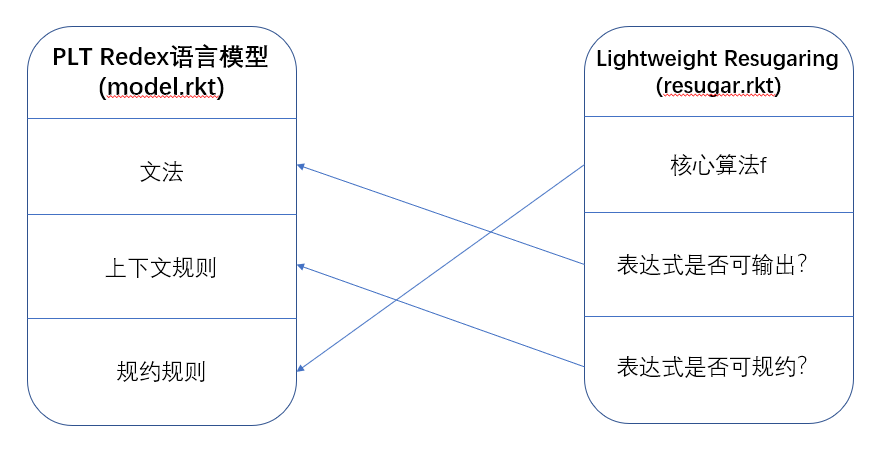
\includegraphics[width=12cm]{images/chapter5/structure.png}
	\caption{程序整体架构}
	\label{fig:struct}
\end{figure}

我们将语言模型(内部语言和外部语言)的文法、上下文规则、规约规则放在model.rkt中,而算法部分放在resugar.rkt中。对于任意新的语法糖,需要进行的修改就是在model.rkt中
\begin{itemize}
	\item 增加对应文法到surfexp
	\item 增加对于上下文规则(让每个子表达式都能进行规约)
	\item 增加语法糖解糖规则到reduction
\end{itemize}
之后在resugar.rkt中构造表达式进行测试即可输出对应重组糖序列。
\section{实现细节}
在PLT Redex中,对一个语言的定义主要需要三个内容。
\begin{itemize}
	\item 文法
	\item 上下文环境
	\item 规约规则
\end{itemize}

我们在实现中,对所有表达式按如下文法进行子类划分。
\begin{verbatim}
exp ::= coreexp | surfexp | commonexp
\end{verbatim}

与(第三章第1节)的定义有所差别的是,这里的surfexp包括了第三章第1节的Surfexp和OtherSurfexp,commonexp包括了第三章第一节的Commonexp和OtherCommonexp。

对于coreexp,自然是包含了所有内部语言的术语。因为我们的定义是将Exp的形式限制在$(Headid\;Subexp_{1}\ldots)$,通常情况下可以根据Headid判断是否是coreexp。

例:
\begin{verbatim}
coreexp ::= (if exp exp exp)
|   (let ((x exp) ...) exp)
|   (first exp)
|   (rest exp)
|   ...
\end{verbatim}

对于surfexp,就是$Headid$是表示DSL的标识的表达式。

例:
\begin{verbatim}
surfexp ::= (and exp exp)
|   (or exp exp)
|   (map exp exp)
|   (filter exp exp)
|   ...
\end{verbatim}

对于commonexp,是为了让我们的重组糖序列中有一些包含在内部语言、但是可以输出的中间过程。例如对于高阶糖

$(Map\;f\;lst)-->(cons\;(f\;(first\;lst))\;(Map\;f\;(rest\;lst)))$

\begin{flushleft}
	我们需要一些中间序列用cons表示,来输出有用的中间过程。我们主要需要的commonexp有所有值、所有基础运算(包括算数运算和列表运算)。
\end{flushleft}

对于上下文规则,对coreLang为了限制每个表达式只有一条规则可以规约,需要仔细限制位置。
而对于surfLang,由于我们不知道哪个子表达式需要先规约,要把每一个位置都设为可规约的洞。
\begin{verbatim}
(E  (v ... E e ...)
(let ((x v) ... (x E) (x e) ...) e)
(if E e e)
(and E e)
(and e E)
(or E e)
(or e E)
...
hole)
\end{verbatim}

规约规则没有特殊说明。具体可参见代码。\footnote{\url{https://github.com/yangdinglou/Lightweight-Resugaring-using-PLT-Redex}}

具体算法实现中,比较复杂的是单步尝试的过程(对应核心算法f的Rule2.2)。因为尽管“检测哪一个子表达式被规约”看起来很容易,实际需要考虑一些极端情况的特例。比如多个子表达式相同,我们不用匹配替代的方法(match/substitute),而是用子表达式替换后检测的方法,将其中一个子表达式替换为一个不可规约的表达式后,检测被规约的子表达式是否发生变化。还有从一个表达式到另一个表达式是否破坏了原表达式的结构,比如从$(and~\#t~(and~\#t~\#t))$到$(and~\#t~\#t)$究竟是破坏了外部语法糖还是对内部子表达式进行规约,都是需要在实现时需要注意的地方。